\RequirePackage{fixltx2e}
\documentclass{jknotes}
\usepackage{joshkirklin}

\begin{document}

\institution{Cambridge Part III Maths}
\title{Advanced Quantum Field Theory}
\lecturer{David Skinner}
\notetaker{Josh Kirklin}
\date{Lent 2016}

\maketitle
\suggestionsspiel
\tableofcontents

\section{Introduction}
\lecture{15/01/16}
We must do three things to construct a QFT:
\begin{enumerate}
    \item Pick a smooth manifold \(\mathcal{M}\) (which we call \emph{space}, or \emph{spacetime} if it is Lorentzian) in which our QFT is going to live, and choose a metric \(g\) for \(\mathcal{M}\).
        For example:
        \begin{itemize}
            \item In particle physics, \(\mathcal{M}=\RR^4\) and \(g=\) the Minkowski metric \(\eta\).
            \item In statistical physics, \(\mathcal{M}=\RR^4\) and \(g=\) the Euclidean metric \(\delta\).
            \item In string theory, \(\mathcal{M}=\Sigma\), some Riemann surface.
        \end{itemize}
    \item Pick some \emph{fields}. These might be:
        \begin{itemize}
            \item Scalar fields \(\phi^a:\mathcal{M}\rightarrow\RR\), \(a=1,\dots,m\). This is known as a \emph{linear sigma model}.
            \item \(\phi:\mathcal{M}\rightarrow\mathcal{N}\) where \((\mathcal{N},G)\) is a general Riemannian manifold. If \(\mathcal{N}\ne \RR^m\), this is called a \emph{non-linear sigma model}.
                \begin{figure}[H]
                    \centering
                    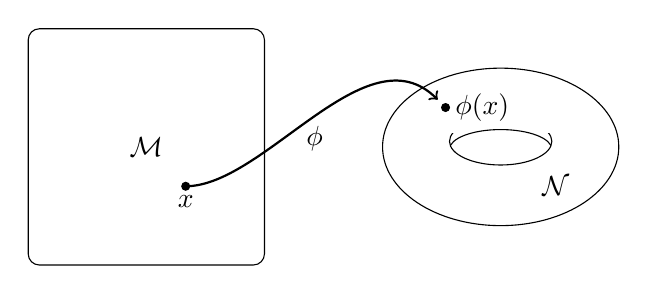
\begin{tikzpicture}
                        \draw[rounded corners](0,0) rectangle (3,3);
                        \node at (1.5,1.5) {\(\mathcal{M}\)};
                        \draw[fill](2,1) circle (0.05) node[below] {\(x\)};

                        \draw(6,1.5) ellipse (1.5 and 1);
                        \begin{scope}
                            \clip(6,1.57) ellipse (0.65 and 0.3);
                            \draw(6,1.47) ellipse (0.65 and 0.25);
                        \end{scope}
                        \begin{scope}
                            \clip(4.5,0) rectangle (7.5,1.67);
                            \draw(6,1.57) ellipse (0.65 and 0.3);
                        \end{scope}
                        \draw[fill](5.3,2) circle (0.05) node[right] {\(\phi(x)\)};
                        \node at (6.7,1) {\(\mathcal{N}\)};

                        \draw[thick,->](2,1) .. controls (3,1) and (4.3,3) .. (5.2,2.1) node[midway, below] {\(\phi\)};
                    \end{tikzpicture}
                \end{figure}
            \item \(\psi\) a (Dirac) spinor on \(\mathcal{M}\).
            \item Gauge fields \(A_\mu(x)\) (taking values in \(\Omega^1(\mathcal{M},\mathcal{L}(G))\), i.e. the set of all 1-forms on \(\mathcal{M}\) with coefficients in the Lie algebra of some Lie group \(G\)).
        \end{itemize}
    \item We must pick an action \(S:\mathcal{C}\rightarrow\RR\), where \(\mathcal{C}\) is the space of fields. For example:
        \begin{itemize}
            \item For a scalar field \(\phi\):
                \begin{equation}
                    S[\phi] = \int_\mathcal{M}\dd[d]{x}\sqrt{g}\Big[ \underbrace{\frac{g^{\mu\nu}}{2}\partial_\mu\phi\partial_\nu\phi}_{\text{kinetic term}}-\underbrace{V(\phi)}_{\mathclap{\substack{\text{potential}\\\text{term}}}} \Big]
                \end{equation}
            \item For a gauge field \(A\):
                \begin{equation}
                    S[A] = \frac{1}{4e^2}\int\dd[d]{x}\sqrt{g}g^{\mu\nu}g^{\rho\sigma}\underbrace{(F_{\mu\rho},F_{\nu\sigma})}_{\text{Killing form}}
                \end{equation}
        \end{itemize}
        In general, the action, even for a scalar, can be the integral of an arbitrary differential polynomial in the fields:
        \begin{equation}
            S[\phi] = \int \underbrace{\mathcal{L}(\phi,\partial^p\phi)}_{\mathclap{\substack{\text{polynomial in }\phi\\\text{and all derivatives}}}} \sqrt{g} \dd[d]{x}
        \end{equation}
\end{enumerate}

\section{QFT in zero dimensions}
If \(\dim \mathcal{M} = 0\) and \(\mathcal{M}\) is connected, then \(\mathcal{M}=\{\text{pt}\}\). We'll choose our fields to be \(\phi:\{\text{pt}\}\rightarrow\RR\) (i.e. \(\phi\in\RR\)).

The basic object we want to compute (in any QFT) is the partition function:
\begin{equation}
    Z = \int_\mathcal{C} \Dd{\phi} e^{-S[\phi]}
\end{equation}
which in this case is just:
\begin{equation}
    Z = \int_\RR \dd{\phi} e^{-S(\phi)}
\end{equation}
We'll assume that \(e^{-S(\phi)}\) decays sufficiently rapidly as \(|\phi|\rightarrow\infty\) that this integral converges. In practice, we take \(S(\phi)\) to be an even degree polynomial in \(\phi\), for example:
\begin{equation}
    S(\phi) = \frac{m^2}{2}\phi^2 + \frac{\lambda}{4!}\phi^4
\end{equation}
In this case \(Z=Z(m,\lambda,\dots)\) is a function of all the coupling constants in \(S(\phi)\). For example:
\begin{equation}
    Z(m^2) = \int_\RR \dd{\phi}e^{-m^2\phi^2/2} = \frac{\sqrt{2\pi}}{m}
\end{equation}
If we include more terms, integrals become hard to solve:
\begin{equation}
    Z(m^2,\phi) = \int_\RR e^{-m^2\phi^2/2-\lambda\phi^4/4!}
\end{equation}
We can try to evaluate this perturbatively in \(\lambda\):
\begin{align}
    Z(m^2,\phi) &= \int \dd{\phi} \left( e^{-m^2\phi^2/2} \sum_{n=0}^\infty \left( \frac{-\lambda}{4!} \right)^n\frac{\phi^{4n}}{n!} \right)\\
    &\stackrel{?}{\sim} \sum_{n=0}^\infty \left( \frac{-\lambda}{4!} \right)^n\frac{1}{n!}\int\dd{\phi}\phi^{4n}e^{-m^2\phi^2/2}
\end{align}
This integral can't possibly converge as a power series in \(\lambda\). In fact this is an asymptotic series\footnote{
    Recall: \(\sum_{n=0}^\infty a_n\lambda^n\) is an asymptotic series for \(Z(\lambda)\) if:
    \begin{equation}
        \lim_{\lambda\rightarrow 0} \frac{|Z(\lambda)-\sum_{n=0}^Na_n\lambda^n|}{\lambda^N}=0 \quad \text{for all } N\in\NN
    \end{equation}
} for \(Z(m^2,\lambda)\). Feynman diagram expansions in QFT are (almost) always asymptotic expansions. It can be shown :
\begin{align}
    Z(m^2\lambda) &\sim \frac{\sqrt{2\pi}}{m}\left[ 1-\frac{\lambda}{8m^4} + \frac{35}{384}\frac{\lambda^2}{m^4} + \dots \right]
\end{align}
Inductively, the coefficient of \(\lambda^n\) is \(\frac{1}{(4!)^nn!}\times\frac{(4n)!}{4^n(2n)!}\). We expect \(\frac{1}{(4!)^nn!}\) as the coefficient in a series expansion. \(\frac{(4n)!}{4^n(2n)!}\) is the number of ways of joining \(4n\) objects into pairs.

\end{document}
